\subsection{Constraint Mapping Performance}
\label{sec:constraintextraction}

Our second experiment evaluates how model and mapper choices affect mapping
quality. We evaluate mapping quality using \emph{constraint extraction} F$_1$ and \emph{aggregate
violation} F$_1$ as metrics. To isolate mapper quality from
classification errors, both metrics are computed only on the ground-truth
constraint sentences. We compare the \emph{Single-Prompt} and \emph{Multi-Step}
mappers across six LLMs on all six datasets.

Figure~\ref{fig:mapper-results} summarizes the results. On the four original
datasets, \emph{Multi-Step} again improves both constraint extraction and
aggregate violation recovery over \emph{Single-Prompt} (mean over models:
0.80 vs.\ 0.75 and 0.89 vs.\ 0.55). The largest gains are on Restaurant and
SISU, whose rules combine several conditions or relate two tuples. Hospital and
Tax are easy for most configurations. With the current backbones, the best
Multi-Step configurations exceed the best configuration of our previous
evaluation (GPT-5, 0.78 extraction and 0.95 violation): Claude Sonnet 5.5 reaches
0.84 and 0.97, and GPT-6 Sol and Mistral Large 4 0.81 and 0.99. Decomposition also keeps the mapper
usable when a backbone is unstable under the single-prompt formulation: a
backbone we initially included, MiniMax-M3, returned empty outputs for most
Single-Prompt batches (107 of 156 sentences counted as output failures) but
completed the Multi-Step pipeline without failures; we replaced it with Mistral
Large 4, and among the six final backbones only DeepSeek-V4-Flash has output
failures (3 Single-Prompt sentences).

\begin{figure}[!ht]
    \centering
    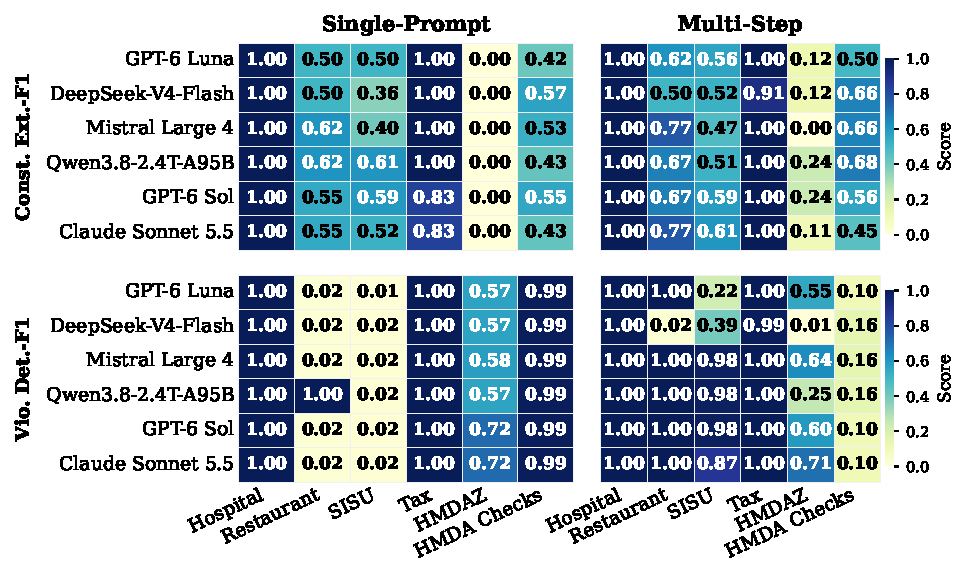
\includegraphics[width=\columnwidth]{figures/results/v3_fig7_mapping.pdf}
    \caption{Sentence-level mapping results across models and mappers, measured by constraint extraction F$_1$ and aggregate violation F$_1$ on ground-truth sentences only.}
    \label{fig:mapper-results}
\end{figure}

\smallskip\noindent\textbf{Where Single-Prompt loses violations.}
The aggregate gap on Restaurant and SISU has two distinct causes. On Restaurant,
one rule (at least one inspection per year) flags 99\% of the gold-violating
tuples. Every Single-Prompt configuration except Qwen3.8-2.4T-A95B returns
\texttt{null} for it, so aggregate recall falls to 0.01. Once this rule is
excluded, all of them reach 1.00. On SISU, the Single-Prompt mapper identifies
the student by the exam registration number instead of the national ID in the
two-tuple rules. The resulting DCs flag about 51k tuples instead of 533
(precision below 0.01), although most single-tuple rules are correct. Multi-Step avoids both errors because it links columns
and selects predicates before writing the DC.

\smallskip\noindent\textbf{HMDA datasets.}
The two HMDA datasets remain the hardest. Exact extraction stays low (at most
0.24 on HMDAZ and 0.68 on HMDA Checks), mainly for two reasons. Many predicted
DCs are logically equivalent to the gold ones but written differently, e.g.,
\texttt{IN} instead of a disjunction, or a label column instead of its code
column. Others omit the coverage conditions of a trigger. Equivalence-aware
extraction (Table~\ref{tab:mapping-metrics}) recovers a large part of the first
group: on the HMDA datasets it raises the mean extraction F$_1$ from 0.36 to
0.49 for Multi-Step and from 0.24 to 0.51 for Single-Prompt. On the four original
datasets it is almost identical to exact extraction. The aggregate violation
ranking is also reversed on HMDA Checks: Single-Prompt reaches 0.99, while
Multi-Step stays at 0.10--0.16. This reversal says little about mapping quality.
Two date-range edits (S270 and Q022) flag 99\% of the gold-violating tuples, which
cover 98.6\% of the rows, so a DC that flags \emph{every} tuple already scores 0.99.
These are the only gold DCs that need arithmetic over dates encoded as integers.
Multi-Step returns \texttt{null} for both with every backbone, consistent with its
precision bias. Single-Prompt writes DCs for them, but most of these DCs flag all
rows (e.g., \texttt{t1.action\_taken\_date / 10000 != t1.activity\_year}, which
never holds as an equality under real division); only GPT-6 Luna, GPT-6 Sol, and
Qwen3.8-2.4T-A95B produce an execution-equivalent DC for one of the two. Without these
two edits, the ranking flips back: Multi-Step reaches 1.00 with Claude Sonnet 5.5,
GPT-6 Luna, and GPT-6 Sol and 0.77 with the other three backbones (mean 0.89),
whereas Single-Prompt ranges from 0.18 to 1.00 (mean 0.65). Per-rule metrics,
which weigh every rule equally, are far less sensitive to these two edits: on
HMDA Checks, the mean per-rule violation F$_1$ is 0.80 for Multi-Step and 0.86 for
Single-Prompt with all edits, and 0.87 and 0.85 without the date edits. On the
remaining rules, the two mappers are therefore close, and the aggregate
reversal does not reflect the overall quality of the rules.

\begin{table}[!ht]
  \centering
  \small
  \setlength{\tabcolsep}{3.5pt}
  \begin{tabular}{llrrrrrr}
\toprule
\textbf{Mapper} & \textbf{Model} & CE & CE$_{\equiv}$ & AV & Rule-F$_1$ & Exec. & Fail. \\
\midrule
\multirow{6}{*}{Single-Prompt} & GPT-6 Luna & 0.57 & 0.69 & 0.60 & 0.78 & 0.75 & 0 \\
 & DeepSeek-V4-Flash & 0.57 & 0.66 & 0.60 & 0.74 & 0.70 & 3 \\
 & Mistral Large 4 & 0.59 & 0.66 & 0.60 & 0.73 & 0.71 & 0 \\
 & Qwen3.8-2.4T-A95B & 0.61 & 0.70 & 0.76 & \textbf{0.86} & \textbf{0.83} & 0 \\
 & GPT-6 Sol & 0.59 & 0.67 & 0.62 & 0.76 & 0.72 & 0 \\
 & Claude Sonnet 5.5 & 0.55 & 0.64 & 0.62 & 0.76 & 0.70 & 0 \\
\midrule
\multirow{6}{*}{Multi-Step} & GPT-6 Luna & 0.63 & 0.68 & 0.65 & 0.75 & 0.73 & 0 \\
 & DeepSeek-V4-Flash & 0.62 & 0.64 & 0.43 & 0.68 & 0.67 & 0 \\
 & Mistral Large 4 & 0.65 & 0.72 & \textbf{0.80} & 0.81 & 0.80 & 0 \\
 & Qwen3.8-2.4T-A95B & \textbf{0.68} & 0.70 & 0.73 & 0.76 & 0.74 & 0 \\
 & GPT-6 Sol & 0.67 & 0.71 & 0.78 & 0.80 & 0.79 & 0 \\
 & Claude Sonnet 5.5 & 0.66 & \textbf{0.73} & 0.78 & 0.84 & 0.81 & 0 \\
\bottomrule
\end{tabular}

  \caption{Mean mapping quality over the six datasets (ground-truth sentences
  only). CE: exact extraction F$_1$; CE$_{\equiv}$: equivalence-aware extraction
  F$_1$; AV: aggregate violation F$_1$; Rule-F$_1$: mean per-rule violation F$_1$;
  Exec.: execution equivalence; Fail.: sentences with no valid model output.}
  \label{tab:mapping-metrics}
\end{table}

\smallskip\noindent\textbf{Default mapper.}
No single model leads on both metrics of the paper protocol: across the six
datasets, Qwen3.8-2.4T-A95B has the best mean extraction (0.68) and Mistral
Large 4 the best mean aggregate violation (0.80) with Multi-Step. We therefore use the mean of the two to break the tie and select
\emph{GPT-6 Sol} with \emph{Multi-Step} (0.67 and 0.78; mean 0.727, against 0.722 for
Mistral Large 4, 0.718 for Claude Sonnet 5.5, and 0.707 for Qwen3.8-2.4T-A95B) as the default
sentence-level configuration. Differences among these four are within the variation that a single
run per configuration can show, so the choice should be read as a tie among
them rather than a clear winner.
\altic{[R1-O11] Aprofundar a análise comparativa entre os foundation models (a figura ``across FMs''): discutir sensibilidade ao modelo, onde e por que modelos divergem, e quais propriedades (tamanho, família, instruction-tuning) correlacionam com desempenho. Hoje a leitura é só ``GPT-5 é melhor''. Isso também ajuda a rebater a sugestão do revisor de mover para track aplicado, mostrando que há achados de método e não só medição.}
